% Kompilacja: pdflatex lagrange.tex
\documentclass[11pt,aspectratio=169]{beamer}

\usepackage[T1]{fontenc}
\usepackage[utf8]{inputenc}
\usepackage{lmodern}
\usepackage[polish]{babel}
\usepackage{amsmath,amssymb,mathtools}
\usepackage{pgfplots}
\pgfplotsset{compat=1.17}
\usetikzlibrary{arrows.meta}
\usepackage{qrcode}

% ---------------------------------------------------------------- wygląd
\definecolor{granat}{RGB}{22,45,90}
\definecolor{akcent}{RGB}{214,105,30}
\definecolor{morski}{RGB}{18,112,112}

\setbeamertemplate{navigation symbols}{}
\setbeamercolor{structure}{fg=granat}
\setbeamercolor{alerted text}{fg=akcent}
\setbeamercolor{item}{fg=akcent}
\setbeamercolor{frametitle}{fg=white,bg=granat}
\setbeamercolor{block title}{fg=white,bg=granat}
\setbeamercolor{block body}{fg=black,bg=granat!7}
\setbeamercolor{block title example}{fg=white,bg=morski}
\setbeamercolor{block body example}{fg=black,bg=morski!8}
\setbeamercolor{footline}{fg=white,bg=granat}
\setbeamercolor{linia}{bg=akcent}
\setbeamertemplate{blocks}[rounded][shadow=true]

\setbeamertemplate{frametitle}{%
  \nointerlineskip
  \begin{beamercolorbox}[wd=\paperwidth,ht=2.6ex,dp=1.1ex,leftskip=1em]{frametitle}%
    \usebeamerfont{frametitle}\insertframetitle
  \end{beamercolorbox}%
  \nointerlineskip
  \begin{beamercolorbox}[wd=\paperwidth,ht=1.5pt,dp=0pt]{linia}\end{beamercolorbox}%
}

\setbeamertemplate{footline}{%
  \begin{beamercolorbox}[wd=\paperwidth,ht=2.4ex,dp=1ex,leftskip=1em,rightskip=1em]{footline}%
    \scriptsize\insertshortauthor\hfill\insertshorttitle\hspace{2em}\insertframenumber\,/\,\inserttotalframenumber
  \end{beamercolorbox}%
}

\newcommand{\wzoran}[1]{\vspace{0.4em}\hfill\fcolorbox{akcent}{akcent!8}{\small$\displaystyle #1$}\par\medskip}

\newtheorem{twierdzenie}{Twierdzenie}
\newenvironment{definicja}{\begin{exampleblock}{Definicja}}{\end{exampleblock}}

% tło ze slajdu tytułowego: portret fazowy (domain coloring) funkcji
% f(z) = (z^2 - 1)(z - 2 - i)^2 / (z^2 + 2 + 2i)
\newcommand{\slajdztlem}[1]{%
  {\usebackgroundtemplate{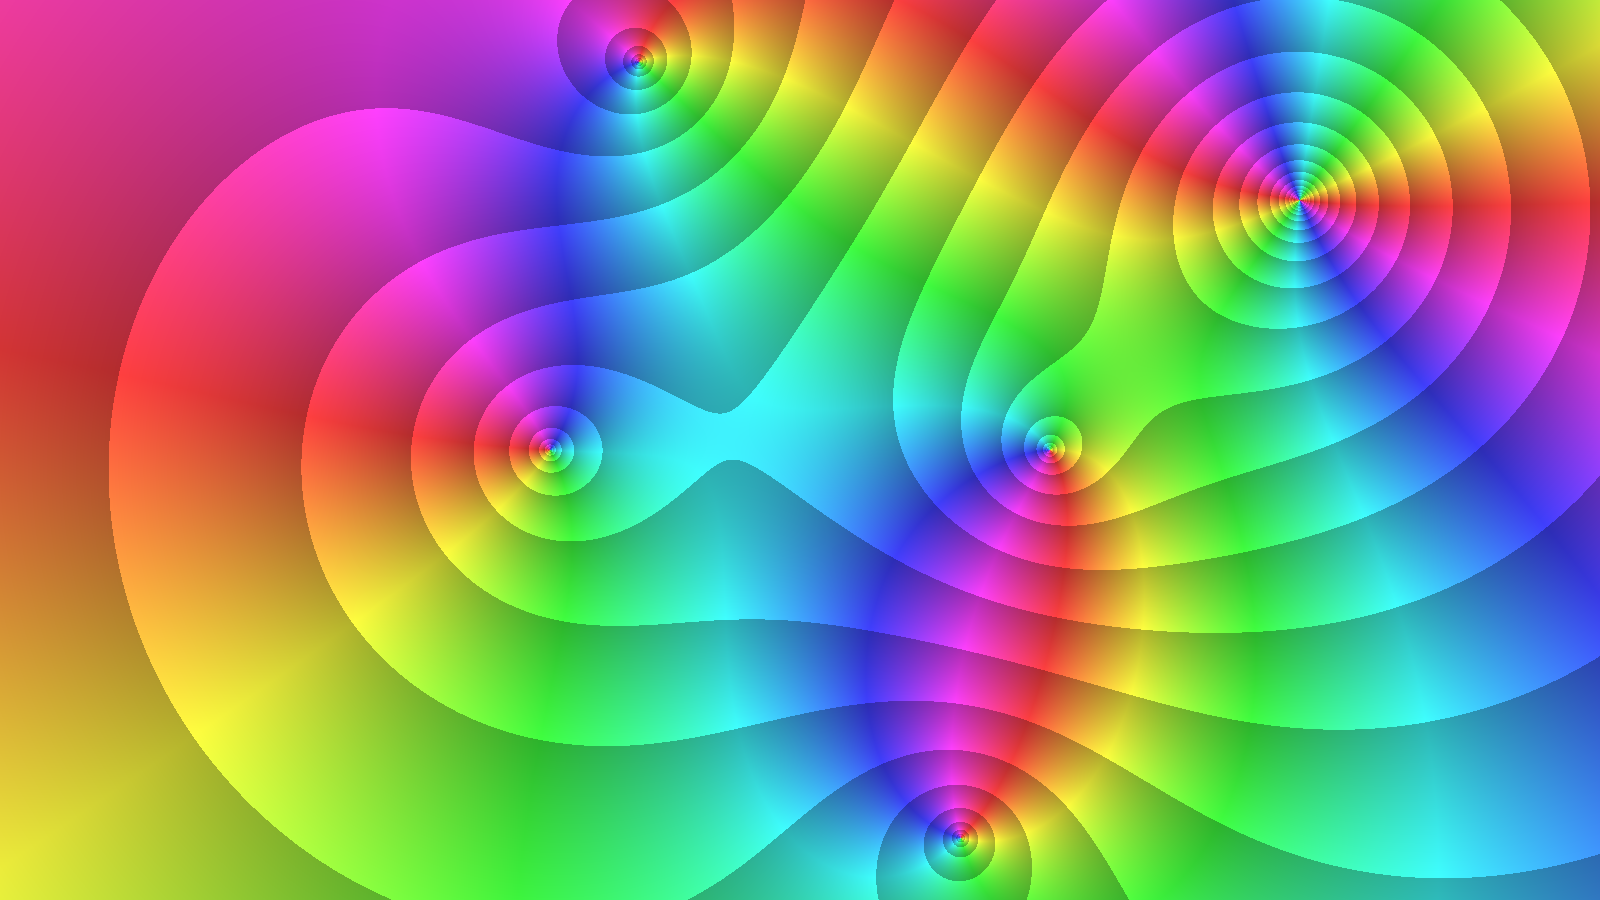
\includegraphics[width=\paperwidth,height=\paperheight]{tlo.png}}%
  \begin{frame}[plain]
    \centering
    \begin{tikzpicture}[remember picture, overlay]
      \node[fill=white, fill opacity=0.88, text opacity=1, rounded corners=6pt, inner sep=14pt, draw=granat, line width=1pt]
        at (current page.center) {\parbox{0.7\paperwidth}{\centering #1}};
    \end{tikzpicture}
  \end{frame}}%
}

\title[Twierdzenie Lagrange'a o odwracaniu]{Twierdzenie Lagrange'a o odwracaniu}
\subtitle{czyli jak odwrócić (prawie) każdą funkcję}
\author{Adrian Madajewski}
\institute{Koło Naukowe Matematyków UAM}
\date{}

\begin{document}

\slajdztlem{%
  {\LARGE\color{granat}\bfseries Twierdzenie Lagrange'a o odwracaniu\par}
  \vspace{0.6em}
  {\large\color{akcent} czyli jak odwrócić (prawie) każdą funkcję\par}
  \vspace{1.4em}
  {\normalsize Adrian Madajewski\par}
  \vspace{0.3em}
  {\small Koło Naukowe Matematyków UAM\par}
}

% ================================================================
\begin{frame}{Problem}
  Mamy funkcję $f$ i równanie
  \[
    f(x) = y .
  \]
  Chcemy wyznaczyć $x$ w zależności od $y$, czyli znaleźć funkcję odwrotną $f^{-1}$.
  \pause
  \bigskip

  Co jeśli nie jesteśmy w stanie znaleźć algebraicznego wzoru na $f^{-1}$?
  \pause
  \bigskip

  Odpowiedź to szeregi potęgowe, czyli funkcje analityczne. Szukamy $f^{-1}$ w postaci
  \[
    f^{-1}(y) = \sum_{n=0}^{\infty} b_n\, (y - y_0)^{n} .
  \]
  \pause
  Pytanie brzmi więc, jak wyznaczyć współczynniki $b_n$.
\end{frame}

% ================================================================
\begin{frame}{Funkcje analityczne}
  \begin{definicja}
    Niech $U \subset \mathbb{C}$ będzie zbiorem otwartym i $\mathbb{N}_0 \coloneqq \{0, 1, 2, \dots\}$. Funkcja $f \colon U \to \mathbb{C}$ jest \emph{analityczna}, jeśli dla każdego $z_0 \in U$ istnieją $r > 0$ oraz ciąg $(a_n)_{n \in \mathbb{N}_0} \subset \mathbb{C}$ takie, że
    \[
      f(z) = \sum_{n=0}^{\infty} a_n\, (z - z_0)^{n}
      \qquad \text{dla } |z - z_0| < r .
    \]
  \end{definicja}
  \pause
  Przykłady
  \[
    e^{z} = \sum_{n=0}^{\infty} \frac{z^{n}}{n!}\ \ (z \in \mathbb{C}),
    \qquad
    \frac{1}{1 - z} = \sum_{n=0}^{\infty} z^{n}\ \ (|z| < 1).
  \]
  \pause
  Interesuje nas rozwinięcie wokół zera, $f(z) = \sum_{n=0}^{\infty} a_n z^{n}$ dla $|z| < R$.
  \medskip

  Jak „wyłuskać'' z funkcji $f$ jeden konkretny współczynnik $a_k$?
\end{frame}

% ================================================================
\begin{frame}{Całka po krzywej}
  \begin{columns}[c]
    \begin{column}{0.6\textwidth}
      Naturalnym rozszerzeniem całki na płaszczyznę zespoloną jest całka po krzywej.
      \medskip

      Krzywą nazywamy odwzorowanie $\gamma \colon [a, b] \to \mathbb{C}$, $\gamma(t) = x(t) + i\, y(t)$, gdzie $x, y \colon [a, b] \to \mathbb{R}$ są klasy $C^{1}$. Kładziemy $\gamma'(t) \coloneqq x'(t) + i\, y'(t)$.
    \end{column}
    \begin{column}{0.38\textwidth}
      \centering
      \begin{tikzpicture}
        \begin{axis}[
          width=5.5cm, height=4.2cm,
          axis lines=middle,
          xmin=-0.3, xmax=4.7, ymin=-0.3, ymax=3.2,
          xtick={1,2,3,4}, ytick={1,2,3},
          tick label style={font=\scriptsize},
          xlabel={$\operatorname{Re} z$}, ylabel={$\operatorname{Im} z$},
          every axis x label/.style={at={(current axis.right of origin)},anchor=south east, font=\scriptsize},
          every axis y label/.style={at={(current axis.above origin)},anchor=north west, font=\scriptsize},
        ]
          \draw[thick, granat, -{Stealth[length=2mm]}] plot[smooth, tension=0.8] coordinates {(0.6,0.6) (1.4,2.1) (2.6,1.2) (3.7,2.5)};
          \addplot[only marks, mark=*, mark size=1.5pt] coordinates {(0.6,0.6) (3.7,2.5)};
          \node[font=\scriptsize, anchor=north west] at (axis cs:0.6,0.6) {$\gamma(a)$};
          \node[font=\scriptsize, anchor=north west] at (axis cs:3.7,2.5) {$\gamma(b)$};
          \node[font=\scriptsize] at (axis cs:1.9,2.2) {$\gamma$};
        \end{axis}
      \end{tikzpicture}
    \end{column}
  \end{columns}
  \pause
  \begin{definicja}
    Dla $f$ ciągłej na $\gamma([a, b])$
    \[
      \int_{\gamma} f(z)\, dz \coloneqq \int_{a}^{b} f\bigl(\gamma(t)\bigr)\, \gamma'(t)\, dt .
    \]
    Gdy $\gamma(a) = \gamma(b)$ (krzywa zamknięta), piszemy $\oint_{\gamma} f(z)\, dz$.
  \end{definicja}
  Część rzeczywistą i urojoną całkujemy osobno.
\end{frame}

% ================================================================
\begin{frame}{Własności całki po krzywej}
  \textbf{Liniowość.} Dla $\alpha, \beta \in \mathbb{C}$
  \[
    \int_{\gamma} \bigl(\alpha f(z) + \beta g(z)\bigr)\, dz = \alpha \int_{\gamma} f(z)\, dz + \beta \int_{\gamma} g(z)\, dz .
  \]
  Wynika wprost z liniowości zwykłej całki $\int_{a}^{b} \dots\, dt$.
  \pause
  \bigskip

  \textbf{Całkowanie przez części po krzywej zamkniętej.} Jeśli $\gamma(a) = \gamma(b)$, to
  \[
    \oint_{\gamma} u(x)\, v'(x)\, dx = - \oint_{\gamma} u'(x)\, v(x)\, dx .
  \]
  Wynika to ze wzoru $\bigl(u(x)\, v(x)\bigr)' = u'(x)\, v(x) + u(x)\, v'(x)$ oraz z tego, że
  \[
    \oint_{\gamma} \bigl(u(x)\, v(x)\bigr)'\, dx = u\bigl(\gamma(b)\bigr)\, v\bigl(\gamma(b)\bigr) - u\bigl(\gamma(a)\bigr)\, v\bigl(\gamma(a)\bigr) = 0 .
  \]
\end{frame}

% ================================================================
\begin{frame}{Parametryzacja okręgu jednostkowego}
  \begin{columns}[c]
    \begin{column}{0.58\textwidth}
      Punkt $z = x + i y$ leży na okręgu jednostkowym, gdy $|z| = 1$, czyli $x^{2} + y^{2} = 1$.
      \pause
      \medskip

      Jeśli $t$ jest kątem między dodatnią półosią rzeczywistą a odcinkiem od $0$ do $z$, to $x = \cos t$ i $y = \sin t$.
      \pause
      Ze wzoru Eulera
      \[
        z = \cos t + i \sin t = e^{it} .
      \]
      \pause
      Gdy $t$ przebiega $[0, 2\pi]$, punkt obiega okrąg raz, przeciwnie do ruchu wskazówek zegara. Zatem
      \[
        \gamma(t) \coloneqq e^{it}, \qquad t \in [0, 2\pi] .
      \]
      \pause
      \vspace{-1.2em}
      \[
        \gamma'(t) = -\sin t + i \cos t = i\,(\cos t + i \sin t) = i e^{it} .
      \]
    \end{column}
    \begin{column}{0.4\textwidth}
      \onslide<1->
      \centering
      \begin{tikzpicture}
        \begin{axis}[
          width=6cm, height=6cm,
          axis lines=middle, axis equal image,
          xmin=-1.6, xmax=1.9, ymin=-1.5, ymax=1.6,
          xtick={-1,1}, ytick={-1,1},
          tick label style={font=\scriptsize},
          xlabel={$\operatorname{Re} z$}, ylabel={$\operatorname{Im} z$},
          every axis x label/.style={at={(current axis.right of origin)},anchor=north east, font=\scriptsize},
          every axis y label/.style={at={(current axis.above origin)},anchor=north west, font=\scriptsize},
        ]
          \addplot[thick, granat, domain=0:360, samples=120] ({cos(x)}, {sin(x)});
          \only<2->{
            \addplot[gray, domain=0:50] ({0.3*cos(x)}, {0.3*sin(x)});
            \addplot[gray] coordinates {(0,0) (0.643,0.766)};
            \addplot[gray, dashed] coordinates {(0.643,0) (0.643,0.766) (0,0.766)};
            \addplot[only marks, mark=*, mark size=1.5pt] coordinates {(0.643,0.766)};
            \node[font=\scriptsize] at (axis cs:0.42,0.18) {$t$};
            \node[font=\scriptsize, anchor=north east] at (axis cs:0.72,0) {$\cos t$};
            \node[font=\scriptsize, anchor=east] at (axis cs:0,0.766) {$\sin t$};
          }
          \only<2>{\node[font=\scriptsize, anchor=south west] at (axis cs:0.643,0.766) {$z$};}
          \only<3->{\node[font=\scriptsize, anchor=south west] at (axis cs:0.643,0.766) {$z = e^{it}$};}
          \only<4->{\addplot[thick, granat, domain=120:145, samples=20, -{Stealth[length=2mm]}] ({cos(x)}, {sin(x)});}
        \end{axis}
      \end{tikzpicture}
    \end{column}
  \end{columns}
\end{frame}

% ================================================================
\begin{frame}{Całka po okręgu jednostkowym}
  \begin{definicja}
    Niech $\gamma(t) = e^{it}$, $t \in [0, 2\pi]$. Dla $f$ ciągłej na okręgu jednostkowym
    \[
      \oint_{|z| = 1} f(z)\, dz \coloneqq \oint_{\gamma} f(z)\, dz = \int_{0}^{2\pi} f\bigl(e^{it}\bigr)\, i e^{it}\, dt .
    \]
  \end{definicja}
\end{frame}

% ================================================================
\begin{frame}{Przykład: $f(z) = z^{p}$, $p \in \mathbb{Z}$}
  W szeregach występują kolejne potęgi $z$, dlatego zaczynamy od nich.
  \pause
  Na okręgu $z = e^{it}$, więc $z^{p} = e^{ipt}$ i
  \[
    \oint_{|z| = 1} z^{p}\, dz
    = \int_{0}^{2\pi} e^{ipt} \cdot i e^{it}\, dt
    = i \int_{0}^{2\pi} e^{i(p+1)t}\, dt .
  \]
  \pause
  Niech $p \neq -1$. Funkcja $\dfrac{e^{i(p+1)t}}{i(p+1)}$ jest pierwotną $e^{i(p+1)t}$, zatem
  \[
    \oint_{|z| = 1} z^{p}\, dz
    = i \left[ \frac{e^{i(p+1)t}}{i(p+1)} \right]_{0}^{2\pi}
    = \frac{e^{2\pi i (p+1)} - e^{0}}{p+1}
    = \frac{1 - 1}{p+1}
    = 0 ,
  \]
  \pause
  bo dla $m \in \mathbb{Z}$ mamy $e^{2\pi i m} = \cos(2\pi m) + i \sin(2\pi m) = 1$.
\end{frame}

% ================================================================
\begin{frame}{Przypadek $p = -1$}
  Wzór ogólny ma w mianowniku $p + 1$, więc dla $p = -1$ nie działa.
  \pause
  Wracamy do rachunku sprzed całkowania
  \[
    \oint_{|z| = 1} z^{-1}\, dz
    = i \int_{0}^{2\pi} e^{i(-1+1)t}\, dt
    = i \int_{0}^{2\pi} 1\, dt
    = 2\pi i .
  \]
  \pause
  \begin{block}{Podsumowanie}
    \[
      \oint_{|z| = 1} z^{p}\, dz =
      \begin{cases}
        2\pi i, & p = -1, \\
        0, & p \in \mathbb{Z} \setminus \{-1\} .
      \end{cases}
    \]
  \end{block}
  \pause
  Spośród wszystkich potęg $z$ tylko $z^{-1}$ ,,przeżywa'' całkowanie po okręgu.
\end{frame}

% ================================================================
\begin{frame}{Pomysł}
  Chcemy odczytać współczynnik przy $z^{k}$. Dzielimy więc przez $z^{k+1}$, aby $z^{k}$ zamieniło się w $z^{-1}$.
  \pause
  \bigskip

  Na przykład dla $f(z) = 3 + 5z + 7z^{2}$ i $k = 1$
  \[
    \frac{f(z)}{z^{2}} = 3 z^{-2} + 5 z^{-1} + 7 ,
    \qquad
    \frac{1}{2\pi i} \oint_{|z| = 1} \frac{f(z)}{z^{2}}\, dz = 3 \cdot 0 + 5 \cdot 1 + 7 \cdot 0 = 5 .
  \]
\end{frame}

% ================================================================
\begin{frame}{Wzór całkowy Cauchy'ego}
  \begin{columns}[c]
    \begin{column}{0.56\textwidth}
      \begin{twierdzenie}[wzór całkowy Cauchy'ego]
        Niech $f(z) = \sum_{n=0}^{\infty} a_n z^{n}$ dla $|z| < R$ i niech $C$ będzie krzywą zamkniętą leżącą w kole $|z| < R$, obiegającą $0$ jeden raz. Wtedy dla każdego $k \in \mathbb{N}_0$
        \[
          a_k = \frac{f^{(k)}(0)}{k!} = \frac{1}{2\pi i} \oint_{C} \frac{f(z)}{z^{k+1}}\, dz .
        \]
      \end{twierdzenie}
    \end{column}
    \begin{column}{0.42\textwidth}
      \centering
      \begin{tikzpicture}
        \begin{axis}[
          width=6.4cm, height=6.4cm,
          axis lines=middle, axis equal image,
          xmin=-2.6, xmax=2.9, ymin=-2.6, ymax=2.7,
          xtick={-2,-1,1,2}, ytick={-2,-1,1,2},
          tick label style={font=\scriptsize},
          xlabel={$\operatorname{Re} z$}, ylabel={$\operatorname{Im} z$},
          every axis x label/.style={at={(current axis.right of origin)},anchor=south east, font=\scriptsize},
          every axis y label/.style={at={(current axis.above origin)},anchor=north west, font=\scriptsize},
        ]
          \addplot[gray, dashed, domain=0:360, samples=120] ({2*cos(x)}, {2*sin(x)});
          \node[font=\scriptsize, gray, anchor=south west] at (axis cs:1.45,1.45) {$|z| = R$};
          \addplot[thick, granat, domain=0:360, samples=300] ({(1.15 + 0.4*sin(5*x) + 0.15*cos(3*x))*cos(x)}, {(1.15 + 0.4*sin(5*x) + 0.15*cos(3*x))*sin(x)});
          \addplot[thick, granat, domain=100:112, samples=20, -{Stealth[length=2mm]}] ({(1.15 + 0.4*sin(5*x) + 0.15*cos(3*x))*cos(x)}, {(1.15 + 0.4*sin(5*x) + 0.15*cos(3*x))*sin(x)});
          \node[font=\scriptsize, anchor=south east] at (axis cs:-1.05,1.0) {$C$};
          \addplot[only marks, mark=*, mark size=1.5pt] coordinates {(0,0)};
          \node[font=\scriptsize, anchor=north east] at (axis cs:0,0) {$0$};
        \end{axis}
      \end{tikzpicture}
    \end{column}
  \end{columns}
\end{frame}

% ================================================================
\begin{frame}{Szukamy funkcji odwrotnej}
  Niech $f$ będzie analityczna w otoczeniu $0$, $f(0) = 0$, $f'(0) \neq 0$.
  Szukamy funkcji odwrotnej $x = x(y)$, czyli takiej, że
  \[
    f\bigl(x(y)\bigr) = y, \qquad x(y) = \sum_{n=0}^{\infty} a_n\, y^{n} = x(0) + \sum_{n=1}^{\infty} a_n\, y^{n} = \sum_{n=1}^{\infty} a_n\, y^{n},
  \]
  bo $f(0) = 0$, więc $x(0) = 0$.
  \pause

  Niech $C$ będzie małą krzywą zamkniętą obiegającą $0$ jeden raz. Ze wzoru Cauchy'ego (zmienną jest teraz $y$) dla $n \ge 1$
  \[
    a_n = \frac{1}{2\pi i} \oint_{f(C)} \frac{x(y)}{y^{n+1}}\, dy .
  \]
  \pause
  Podstawiamy $y = f(x)$. Gdy $x$ obiega $C$, $y = f(x)$ obiega $f(C)$, oraz $dy = f'(x)\, dx$. Zatem
  \[
    \boxed{\; a_n = \frac{1}{2\pi i} \oint_{C} \frac{x\, f'(x)}{f(x)^{n+1}}\, dx \;}
  \]
\end{frame}

% ================================================================
\begin{frame}[t]{Funkcja $\varphi$}
  \wzoran{a_n = \frac{1}{2\pi i} \oint_{C} \frac{x\, f'(x)}{f(x)^{n+1}}\, dx}
  Załóżmy, że
  \[
    f(x) = \frac{x}{\varphi(x)}
  \]
  dla pewnej funkcji $\varphi$ analitycznej w otoczeniu $0$, takiej że $\varphi(0) \neq 0$.
  \pause
  \medskip

  Wtedy
  \[
    f'(x) = \frac{\varphi(x) - x\, \varphi'(x)}{\varphi(x)^{2}},
    \qquad
    f(x)^{n+1} = \frac{x^{n+1}}{\varphi(x)^{n+1}} .
  \]
  \pause
  W szczególności $f'(0) = \dfrac{\varphi(0)}{\varphi(0)^{2}} = \dfrac{1}{\varphi(0)}$, więc warunek $\varphi(0) \neq 0$ to dokładnie założenie $f'(0) \neq 0$.
\end{frame}

% ================================================================
\begin{frame}{Upraszczamy}
  \wzoran{a_n = \frac{1}{2\pi i} \oint_{C} \frac{x\, f'(x)}{f(x)^{n+1}}\, dx}
  Wstawiamy do funkcji podcałkowej
  \[
    \frac{x\, f'(x)}{f(x)^{n+1}}
    = x \cdot \frac{\varphi(x) - x\, \varphi'(x)}{\varphi(x)^{2}} \cdot \frac{\varphi(x)^{n+1}}{x^{n+1}}
    = \frac{\varphi(x)^{n-1} \bigl(\varphi(x) - x\, \varphi'(x)\bigr)}{x^{n}} .
  \]
  \pause
  Rozbijamy na dwa składniki
  \[
    \frac{\varphi(x)^{n-1} \bigl(\varphi(x) - x\, \varphi'(x)\bigr)}{x^{n}}
    = \frac{\varphi(x)^{n}}{x^{n}} - \frac{\varphi(x)^{n-1}\, \varphi'(x)}{x^{n-1}} .
  \]
  \pause
  Zatem $a_n = I_1 - I_2$, gdzie
  \[
    I_1 \coloneqq \frac{1}{2\pi i} \oint_{C} \frac{\varphi(x)^{n}}{x^{n}}\, dx ,
    \qquad
    I_2 \coloneqq \frac{1}{2\pi i} \oint_{C} \frac{\varphi(x)^{n-1}\, \varphi'(x)}{x^{n-1}}\, dx .
  \]
\end{frame}


% ================================================================
\begin{frame}{Druga całka}
  \wzoran{a_n = I_1 - I_2, \qquad I_2 = \frac{1}{2\pi i} \oint_{C} \frac{\varphi(x)^{n-1}\, \varphi'(x)}{x^{n-1}}\, dx}
  Podstawienie $u = \varphi(x)$, $du = \varphi'(x)\, dx$:
  \[
    I_2 = \frac{1}{2\pi i} \oint_{C} \frac{1}{x^{n-1}}\, u^{n-1}\, du .
  \]
  \pause
  Podstawienie $w = u^{n}$, $dw = n\, u^{n-1}\, du$, czyli $u^{n-1}\, du = \frac{1}{n}\, d\bigl(\varphi(x)^{n}\bigr)$:
  \[
    I_2 = \frac{1}{n} \cdot \frac{1}{2\pi i} \oint_{C} \frac{1}{x^{n-1}}\, d\bigl(\varphi(x)^{n}\bigr) .
  \]
  \pause
  Przez części z $u = \dfrac{1}{x^{n-1}}$, $v = \varphi(x)^{n}$, gdzie $\left(\dfrac{1}{x^{n-1}}\right)' = -\dfrac{n-1}{x^{n}}$:
  \[
    I_2 = -\frac{1}{n} \cdot \frac{1}{2\pi i} \oint_{C} \varphi(x)^{n} \left(\frac{1}{x^{n-1}}\right)' dx
        = \frac{n-1}{n} \cdot \frac{1}{2\pi i} \oint_{C} \frac{\varphi(x)^{n}}{x^{n}}\, dx
        = \frac{n-1}{n}\, I_1 .
  \]
\end{frame}

% ================================================================
\begin{frame}{Twierdzenie Lagrange'a}
  \wzoran{I_1 = \frac{1}{2\pi i} \oint_{C} \frac{\varphi(x)^{n}}{x^{n}}\, dx, \qquad I_2 = \frac{n-1}{n}\, I_1}
  Mamy więc
  \[
    a_n = I_1 - \frac{n-1}{n}\, I_1 = \frac{1}{n}\, I_1 = \frac{1}{n} \cdot \frac{1}{2\pi i} \oint_{C} \frac{\varphi(x)^{n}}{x^{n}}\, dx .
  \]
  \pause
  Ostatnia całka to wzór Cauchy'ego dla funkcji $\varphi^{n}$ i $k = n - 1$.
  \pause
  \begin{twierdzenie}[Lagrange]
    Niech $f$ będzie analityczna w otoczeniu $0$, $f(0) = 0$, $f'(0) \neq 0$, i niech $\varphi(x) \coloneqq x / f(x)$. Wtedy w pewnym otoczeniu $0$ funkcja odwrotna ma rozwinięcie $x(y) = \sum_{n=1}^{\infty} a_n y^{n}$, gdzie
    \[
      a_n = \frac{1}{n!}\, \frac{d^{\,n-1}}{dx^{\,n-1}} \Bigl[ \varphi(x)^{n} \Bigr]_{x = 0}, \qquad n \ge 1 .
    \]
  \end{twierdzenie}
\end{frame}

% ================================================================
\begin{frame}{Przykład: $f(x) = \frac{x}{1 + x}$}
  \wzoran{a_n = \frac{1}{n!}\, \frac{d^{\,n-1}}{dx^{\,n-1}} \Bigl[ \varphi(x)^{n} \Bigr]_{x = 0}, \qquad \varphi(x) = \frac{x}{f(x)}}
  \textbf{Znamy odwrotność.} Z $y = \dfrac{x}{1 + x}$ mamy $y + yx = x$, czyli
  \[
    x(y) = \frac{y}{1 - y} = y + y^{2} + y^{3} + \dots \qquad (|y| < 1)
  \]
  \pause
  \textbf{Sprawdzamy twierdzenie.} $\varphi(x) = \dfrac{x}{f(x)} = 1 + x$, więc $\varphi(x)^{n} = (1 + x)^{n}$.
  \pause
  \begin{itemize}
    \item $n = 1$: $\quad a_1 = \dfrac{1}{1!}\, (1 + 0) = 1$. \quad $\checkmark$
    \pause
    \item $n = 2$: $\quad \dfrac{d}{dx} (1 + x)^{2} = 2\, (1 + x)$, więc $a_2 = \dfrac{1}{2!} \cdot 2 = 1$. \quad $\checkmark$
    \pause
    \item $n = 3$: $\quad \dfrac{d^{2}}{dx^{2}} (1 + x)^{3} = 6\, (1 + x)$, więc $a_3 = \dfrac{1}{3!} \cdot 6 = 1$. \quad $\checkmark$
  \end{itemize}
\end{frame}

% ================================================================
\begin{frame}{Przykład: $f(x) = x e^{x}$}
  \wzoran{a_n = \frac{1}{n!}\, \frac{d^{\,n-1}}{dx^{\,n-1}} \Bigl[ \varphi(x)^{n} \Bigr]_{x = 0}, \qquad \varphi(x) = \frac{x}{f(x)}}
  Mamy $f(0) = 0$ i $f'(0) = 1 \neq 0$. Odwrotności do $y = x e^{x}$ nie da się wyrazić wzorem algebraicznym. Nazywa się ją funkcją $W$ Lamberta.
  \pause
  \medskip

  $\varphi(x) = \dfrac{x}{x e^{x}} = e^{-x}$, więc $\varphi(x)^{n} = e^{-nx}$ oraz
  \[
    \frac{d^{\,n-1}}{dx^{\,n-1}}\, e^{-nx} = (-n)^{n-1}\, e^{-nx} .
  \]
  \pause
  Stąd
  \[
    a_n = \frac{(-n)^{n-1}}{n!},
    \qquad
    W(y) = \sum_{n=1}^{\infty} \frac{(-n)^{n-1}}{n!}\, y^{n} = y - y^{2} + \frac{3}{2}\, y^{3} - \frac{8}{3}\, y^{4} + \dots
  \]
\end{frame}

% ================================================================
\begin{frame}{Gdzie szereg $W$ jest zbieżny?}
  \wzoran{W(y) = \sum_{n=1}^{\infty} a_n\, y^{n}, \qquad a_n = \frac{(-n)^{n-1}}{n!}}
  Kryterium d'Alemberta:
  \[
    \frac{|a_{n+1}|}{|a_n|}
    = \frac{(n+1)^{n}}{(n+1)!} \cdot \frac{n!}{n^{n-1}}
    = \frac{(n+1)^{n-1}}{n^{n-1}}
    = \left(1 + \frac{1}{n}\right)^{n-1}
    \xrightarrow[n \to \infty]{} e .
  \]
  \pause
  Promień zbieżności wynosi więc
  \[
    R = \frac{1}{e}, \qquad \text{czyli szereg jest zbieżny dla } |y| < \frac{1}{e} .
  \]
  \pause
  Dlaczego akurat $\frac{1}{e}$? Dla $f(x) = x e^{x}$ mamy $f'(x) = (1 + x)\, e^{x}$, więc $f'(-1) = 0$ i $f(-1) = -\frac{1}{e}$. W punkcie $y = -\frac{1}{e}$ funkcja odwrotna przestaje istnieć lokalnie, więc szereg nie może sięgać dalej.
\end{frame}

% ================================================================
\begin{frame}{Ogólna wersja twierdzenia}
  Dotąd rozwijaliśmy w zerze, $f(0) = 0$. Niech teraz $f(a) = b$, $f'(a) \neq 0$.
  \pause
  \medskip

  Kładziemy $g(t) \coloneqq f(t + a) - b$. Wtedy $g(0) = 0$, $g'(0) = f'(a) \neq 0$, a
  \[
    y = f(x) \iff y - b = g(x - a) .
  \]
  Stosujemy twierdzenie do $g$ w zmiennych $t = x - a$ oraz $y - b$.
  \pause
  \begin{twierdzenie}[Lagrange, wersja ogólna]
    Niech $f$ będzie analityczna w otoczeniu $a$, $f(a) = b$, $f'(a) \neq 0$. Wtedy w pewnym otoczeniu $b$
    \[
      x(y) = a + \sum_{n=1}^{\infty} \frac{(y - b)^{n}}{n!}\, \frac{d^{\,n-1}}{dx^{\,n-1}} \left[ \left( \frac{x - a}{f(x) - b} \right)^{n} \right]_{x = a} .
    \]
  \end{twierdzenie}
\end{frame}

% ================================================================
\slajdztlem{%
  {\LARGE\color{granat}\bfseries Dziękuję za uwagę!\par}
  \vspace{1em}
  \colorbox{white}{\qrcode[height=2.6cm]{https://github.com/AdrianMadajewski/lagrange-inversion-theorem}}\par
  \vspace{0.5em}
  {\scriptsize\texttt{github.com/AdrianMadajewski/lagrange-inversion-theorem}\par}
}

% ================================================================
\begin{frame}{Literatura}
  \begin{itemize}
    \item F.~Leja, \emph{Funkcje zespolone}, PWN, Warszawa.
    \item J.~Chądzyński, \emph{Wstęp do analizy zespolonej}, PWN, Warszawa, 1999.
    \item W.~Rudin, \emph{Analiza rzeczywista i zespolona}, PWN, Warszawa.
    \item E.\,M.~Stein, R.~Shakarchi, \emph{Complex Analysis}, Princeton University Press, 2003.
    \item \emph{Lagrange inversion theorem}, Wikipedia (wersja angielska).
  \end{itemize}
\end{frame}

\end{document}
